\documentclass[finalReport.tex]{subfiles}
\begin{document}

\chapter{Requirements and Design}\label{ch:r-d}


This section describes the software design of the client and server entities according to the Software Engineering Paradigm Unified Modeling Language (UML) standardization.

Initially, the functional requirements for the server side (Section \ref{sec:FRserver}) and the client side (\ref{sec:FRclient}) are presented. Then the Use Cases (Section \ref{sec_UC}) are identified and mapped to the functional requirements previously identified (Section \ref{sec:mapping}). In conclusion, some general notes are presented (Section \ref{sec:notes}). 


\section{Functional Requirements of the Server}\label{sec:FRserver} 
In order to have an optimal development of the project, the following functional requirements from the Server side are identified:
\begin{enumerate}[label=(\Alph*)]

\item the server is able to listen for connections from remote clients
\begin{enumerate}[label=(\Alph*)]
\item the server starts a new thread 
\end{enumerate}

\item the server is able to query a database
\begin{enumerate}[label=(\Alph*)]
\item to check the existence of a username
\item to check the matching of username and password
\item to update the information of a user inside the database
\item to select information about a user
\item to insert a new contact-relationship between two users
\item to select all the contacts of a user
\end{enumerate} 

\item the server is able to reply to the client's requests
\begin{enumerate}[label=(\Alph*)]
\item to allow the registration of a new user
\item to allow the login of a user
\item to update the connection details of a user inside the database
\item to provide information about a second user
\item to pair two users as contacts
\item to provide the user her list of contacts
\item to allow the logout 
\end{enumerate}


\end{enumerate}




\section{Functional Requirements of the Client} \label{sec:FRclient} 
In order to have an optimal development of the project, the following functional requirements from the Client side are identified:
\begin{enumerate}[label=(\alph*)]

\item the user is able to log in the application \label{item:login}
\begin{enumerate}[label=(\alph*)]
\item the user inserts her credential
\item the user accesses her personalised main page
\end{enumerate}

\item a new user is able to register herself in the application
\begin{enumerate}[label=(\alph*)]
\item the user inserts her new credentials
\item the user accesses a standard main page
\end{enumerate}

\item the user is able to add a contact
\begin{enumerate}[label=(\alph*)]
\item the user looks for another user
\item the user sees the new contact displayed in her contacts page
\end{enumerate}

\item the user is able to start a chat with another user
\begin{enumerate}[label=(\alph*)]
	\item the user starts the connection
	\item the user opens a new chat tab
\begin{enumerate}[label=(\alph*)]
		\item the contacted user's chat tab is opened automatically 
\end{enumerate}
	\item the user sends and receives messages
\end{enumerate}

\item the user is able to leave the application \label{item:logout}
\begin{enumerate}
\item the user closes all her connections
\end{enumerate}

\item \textit{the user is able to use a secure connection}\label{item:secure}
\item \textit{the user is able to set a status, a name and a display picture}\label{item:pers}
\item \textit{the user is able to delete her account}
\item \textit{the user is able to send emojis and pictures}
\item \textit{the user is able to back up her conversation}
\item \textit{the user is able to remove a sent message}
\item \textit{the user is able to customise the aspect of her interface}\label{item:pers2}

\end{enumerate}

The requirements from \ref{item:login} to \ref{item:logout} were considered mandatory in the first phase of the software's design, with the only exception of the availability of a contact list for each user: these all have been implemented.
  
The item \ref{item:secure} was classified as mandatory, but it has not been implemented, as have not the items from \ref{item:pers} to \ref{item:pers2} in italics. 





\section{Use Cases}\label{sec_UC} 
The Use Cases explain how the actors can interact with the system. In this project the actors are different instances of \textit{Clients}.

Below all the modelled Use Cases (Figure \ref{Fig: UC}) are presented:

\begin{enumerate}
\item Login \label{UC:login}
\begin{itemize}
\item[1.1] Get contacts \label{UC:get_contacts}
\end{itemize}
\item Registration \label{UC:registration}
\item Add a contact \label{UC:add_contact}
\begin{itemize}
\item[3.1] Search a contact \label{UC:search_contact}
\end{itemize}
\item Start a chat \label{UC:start_chat}
\begin{itemize}
\item[4.1] Start a connection \label{UC:connection}
\item[4.2] Conversation	\label{UC:conversation}
\end{itemize}
\item Close the application \label{UC:close}
\begin{itemize}
\item[5.1] Logout \label{UC:logout}
\end{itemize}
\end{enumerate}

Further details about the Use Cases are available in the Appendix \ref{app:uc}.

\begin{figure}[h] 
\centering
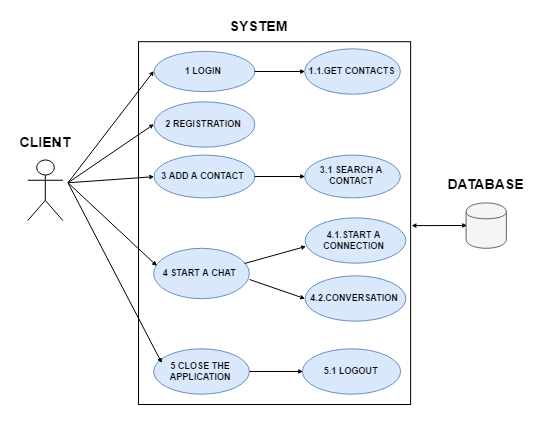
\includegraphics[scale=0.75]{RandD/Plot/UMLusecases.png}
\caption{Use Cases UML Diagram}\label{Fig: UC}
\end{figure}



\clearpage



\clearpage
\section{Mapping Functional Requirements to Use Cases}\label{sec:mapping}

Tables \ref{Tab:FRvsUC_server} and \ref{Tab:FRvsUC_client} show the relation between the Use Cases and the Functional Requirements, respectively, of the Server and the Client. The optional Requirements identified in the first phase of the project's design have not been mapped to any Use Case and have not been implemented.

\begin{table}[h]\centering
\begin{tabular}{|c|c|c|c|c|c|c|c|c|c|c|}
\hline 
 & \textbf{1} & 1.1 & \textbf{2} & \textbf{3} & 3.1 & \textbf{4} & 4.1 & 4.2 & \textbf{5} & 5.1 \\ 
\hline 
\textbf{A} & x & x &  &  &  &  &  &  &  &  \\ 
\hline 
A.A & x & x &  &  &  &  &  &  &  &  \\ 
\hline 
\textbf{B} & x & x & x & x & x & x & x &  & x & x \\ 
\hline 
B.A &  &  & x &  &  &  &  &  &  &  \\ 
\hline 
B.B & x &  &  &  &  &  &  &  &  &  \\ 
\hline 
B.C & x &  &  &  &  &  &  &  & x & x \\ 
\hline 
B.D &  &  &  & x & x & x & x &  &  &  \\ 
\hline 
B.E &  &  &  & x &  &  &  &  &  &  \\ 
\hline 
B.F &  & x &  &  &  &  &  &  &  &  \\ 
\hline 
\textbf{C} & x & x & x & x & x & x & x &  & x & x \\ 
\hline 
C.A &  &  & x &  &  &  &  &  &  &  \\ 
\hline 
C.B & x &  &  &  &  &  &  &  &  &  \\ 
\hline 
C.C & x &  &  &  &  &  &  &  &  &  \\ 
\hline 
C.D &  &  &  & x & x & x & x &  &  &  \\ 
\hline 
C.E &  &  &  & x &  &  &  &  &  &  \\ 
\hline 
C.F &  & x &  &  &  &  &  &  &  &  \\ 
\hline 
C.G &  &  &  &  &  &  &  &  &  & x \\ 
\hline 
\end{tabular} 
\caption{Mapping between the Functional Requirements of the Server and the Use Cases.}\label{Tab:FRvsUC_server}
\end{table}


\begin{table}\centering
\begin{tabular}{|c|c|c|c|c|c|c|c|c|c|c|}
\hline 
 & \textbf{1} & 1.1 & \textbf{2} & \textbf{3} & 3.1 & \textbf{4} & 4.1 & 4.2 & \textbf{5} & 5.1 \\ 
\hline 
\textbf{a} & x & x &  &  &  &  &  &  &  &  \\ 
\hline 
a.a & x &  &  &  &  &  &  &  &  &  \\ 
\hline 
a.b & x & x &  &  &  &  &  &  &  &  \\ 
\hline 
\textbf{b} &  &  & x &  &  &  &  &  &  &  \\ 
\hline 
b.a &  &  & x &  &  &  &  &  &  &  \\ 
\hline 
b.b &  &  & x &  &  &  &  &  &  &  \\ 
\hline 
\textbf{c} &  &  &  & x & x &  &  &  &  &  \\ 
\hline 
c.a &  &  &  & x & x &  &  &  &  &  \\ 
\hline 
c.b &  &  &  & x &  &  &  &  &  &  \\ 
\hline 
\textbf{d} &  &  &  &  &  & x & x & x &  &  \\ 
\hline 
d.a &  &  &  &  &  & x & x &  &  &  \\ 
\hline 
d.b &  &  &  &  &  & x & x &  &  &  \\ 
\hline 
d.b.a &  &  &  &  &  & x & x &  &  &  \\ 
\hline 
d.c &  &  &  &  &  & x &  & x &  &  \\ 
\hline 
\textbf{e} &  &  &  &  &  &  &  &  & x & x \\ 
\hline 
e.a &  &  &  &  &  &  &  &  &  & x \\ 
\hline 
\end{tabular} 
\caption{Mapping between the Functional Requirements of the Cllient and the Use Cases.}\label{Tab:FRvsUC_client}
\end{table}


\section{General notes}\label{sec:notes}

\subsection{Socket Programming}
It was ultimately decided to employ sockets to develop the application, since the other methods employ several layers of abstraction. Socket programming allows the project team to implement network communication as close as possible to the operating system without rewriting the network stack. The effect of designing the application using sockets eventually required the team to implement a multi-threaded implementation.


\subsection{Database Design}

As mentioned earlier, the database design was modified as with the local copy of the database it was not possible for any other client to login from a remote machine.This was due to the fact that the remote clients contacts were stored locally.This issue was solved by storing the database on the server side.By doing this we also made the application more efficient. 
There are two tables in the chat server database-'users' and 'contacts'. The users table has the following fields;  username,password,connection and date with username as the primary key. The contacts table has the following fields; username and contacts where both are primary keys. 

\begin{figure}[h] 
\centering
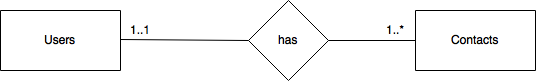
\includegraphics[scale=0.75]{db.png}
\caption{Entity-Relation Diagram for the Database}\label{db}
\end{figure}



\end{document}